\documentclass[tikz,border=3pt]{standalone}
\usepackage{amsmath,amssymb,bm}
\usetikzlibrary{arrows.meta,calc,positioning}

\definecolor{JunctionWater}{HTML}{1676B7}
\definecolor{JunctionWall}{HTML}{303030}
\definecolor{JunctionGuide}{HTML}{8B8B8B}

\begin{document}
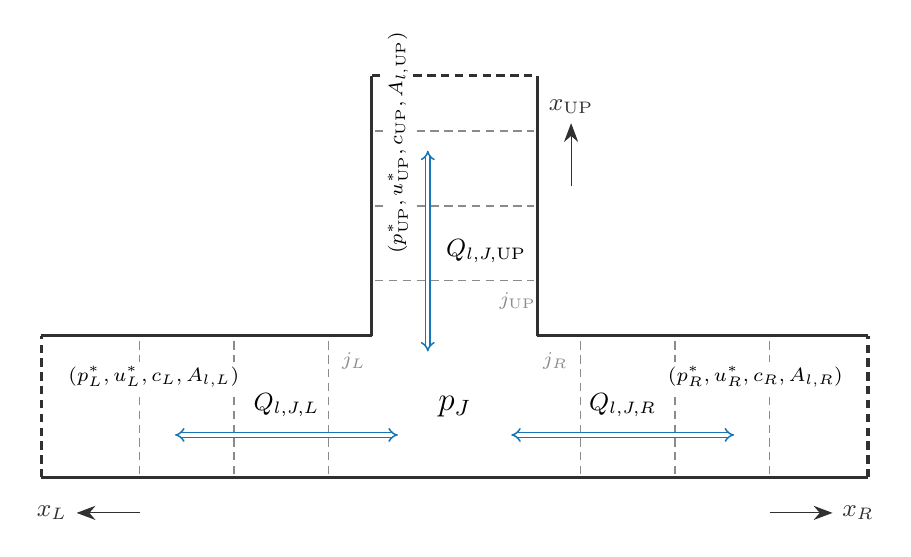
\begin{tikzpicture}[
  x=1cm,y=1cm,
  >=Stealth,
  pipe/.style={draw=JunctionWall,line width=1.15pt},
  pipeend/.style={draw=JunctionWall,densely dashed,line width=1.15pt},
  gridface/.style={draw=JunctionGuide,densely dashed,line width=0.55pt},
  liquid/.style={draw=JunctionWater,line width=1.65pt,-{Stealth[length=3.2mm,width=2.2mm]}},
  liquiddouble/.style={draw=JunctionWater,line width=0.55pt,double=white,
    double distance=1.15pt,
    {Implies[length=3.8mm,width=3.0mm]}-{Implies[length=3.8mm,width=3.0mm]}},
  trace/.style={font=\scriptsize,fill=white,inner sep=1.5pt},
  branch/.style={font=\small}
]
  % Open T-shaped pipe walls.
  \draw[pipe] (-5.25,-0.90) -- (5.25,-0.90);
  \draw[pipe] (-5.25, 0.90) -- (-1.05,0.90);
  \draw[pipe] ( 1.05, 0.90) -- ( 5.25,0.90);
  \draw[pipeend] (-5.25,-0.90) -- (-5.25,0.90);
  \draw[pipeend] ( 5.25,-0.90) -- ( 5.25,0.90);
  \draw[pipe] (-1.05,0.90) -- (-1.05,4.20);
  \draw[pipe] ( 1.05,0.90) -- ( 1.05,4.20);
  \draw[pipeend] (-1.05,4.20) -- (1.05,4.20);

  % Cell faces belong to the three one-dimensional branches; the central
  % junction itself has no finite-volume storage.
  \foreach \x in {-4.0,-2.8,-1.6,1.6,2.8,4.0}
    \draw[gridface] (\x,-0.86) -- (\x,0.86);
  \foreach \y in {1.60,2.55,3.50}
    \draw[gridface] (-1.01,\y) -- (1.01,\y);
  \node[font=\scriptsize,text=JunctionGuide] at (-1.28,0.58) {$j_L$};
  \node[font=\scriptsize,text=JunctionGuide] at ( 1.28,0.58) {$j_R$};
  \node[font=\scriptsize,text=JunctionGuide] at (0.80,1.34) {$j_{\mathrm{UP}}$};

  % Massless junction node.
  \node[font=\large] at (0,0) {$p_J$};

  % Signed liquid discharges; positive directions follow the branch coordinates.
  \draw[liquiddouble] (-0.72,-0.36) -- (-3.55,-0.36)
    node[midway,above=3pt,font=\small] {$Q_{l,J,L}$};
  \draw[liquiddouble] (0.72,-0.36) -- (3.55,-0.36)
    node[midway,above=3pt,font=\small] {$Q_{l,J,R}$};
  \draw[liquiddouble] (-0.34,0.70) -- (-0.34,3.25)
    node[midway,right=3pt,font=\small] {$Q_{l,J,\mathrm{UP}}$};

  % Adjacent branch traces and branch identifiers.
  \node[trace] at (-3.82,0.38)
    {$(p_L^*,u_L^*,c_L,A_{l,L})$};
  \node[trace] at (3.82,0.38)
    {$(p_R^*,u_R^*,c_R,A_{l,R})$};
  \node[trace,rotate=90] at (-0.72,3.35)
    {$(p_{\mathrm{UP}}^*,u_{\mathrm{UP}}^*,c_{\mathrm{UP}},A_{l,\mathrm{UP}})$};
  % Coordinate directions coincide with positive branch directions.
  \draw[JunctionWall,thin,-{Stealth[length=2.4mm]}] (-4.00,-1.35) -- (-4.80,-1.35)
    node[left,font=\small] {$x_L$};
  \draw[JunctionWall,thin,-{Stealth[length=2.4mm]}] (4.00,-1.35) -- (4.80,-1.35)
    node[right,font=\small] {$x_R$};
  \draw[JunctionWall,thin,-{Stealth[length=2.4mm]}] (1.48,2.80) -- (1.48,3.60)
    node[above,font=\small] {$x_{\mathrm{UP}}$};
\end{tikzpicture}
\end{document}
